\documentclass[10pt,a4paper]{article}
\usepackage{amsmath,amssymb,amsthm,graphicx}
\usepackage{fullpage}
\usepackage{authblk}
\usepackage[draft]{hyperref} 
\usepackage{graphicx,amsfonts} % Required for inserting images
\usepackage{tikz}
\usepackage{algorithm} % nicematrix unused in author body; omitted locally.
\usepackage[noend]{algpseudocode}

\usepackage{xcolor}
\usepackage{multirow}

% \hypersetup{
%     colorlinks=true,
%     allcolors=blue,
% }
\usepackage[capitalize,noabbrev]{cleveref}

\usepackage{amsmath,amssymb,amsthm}
\usepackage{thmtools}
\usepackage{thm-restate}

\usetikzlibrary{patterns,tikzmark}
\usetikzlibrary{matrix,decorations.pathreplacing,calc,fit,backgrounds,calligraphy}

% Redefine comments to be gray and italic
\algrenewcommand\algorithmiccomment[1]{\hfill\textit{\textcolor{gray}{{ $\triangleright$  #1}}}}
% \algrenewcommand\keyword{new name}

\newtheorem{theorem}{Theorem}[section]
\newtheorem{corollary}{Corollary}[theorem]
\newtheorem{lemma}[theorem]{Lemma}
\newtheorem{remark}[theorem]{Remark}
\newtheorem{observation}[theorem]{Observation}

\newcommand{\field}{\mathbb{F}}
\newcommand{\matsize}[2]{#1\times #2}
\newcommand{\matexp}{\omega}
\newcommand{\X}{\mathbb{X}}
\newcommand{\dgm}{\mathrm{dgm}}
\newcommand{\mat}[1]{\mathbf{#1}}
\newcommand{\bdr}{\mat{D}}
\newcommand{\PH}{PH}

\newcommand{\low}{\mathbf{low}}
\newcommand{\lft}{\mathbf{lft}}

\newcommand{\Remark}[1]{\textcolor{blue}{[#1]}}
\newcommand{\primoz}[1]{\textcolor{red}{[#1]}}
\newcommand{\fix}[1]{\textcolor{red}{[#1]}}

%\renewcommand{\paragraph}[1]{\subparagraph*{#1.}}
\renewcommand{\paragraph}[1]{\noindent\textbf{#1.}}


\DeclareMathOperator*{\argmin}{arg\,min}
\DeclareMathOperator*{\argmax}{arg\,max}

\pgfmathsetmacro{\myscale}{2}
\pgfkeys{tikz/mymatrixenv/.style={decoration={brace},every left delimiter/.style={xshift=8pt},every right delimiter/.style={xshift=-8pt}}}
\pgfkeys{tikz/mymatrix/.style={matrix of math nodes,nodes in empty cells,
left delimiter={[},right delimiter={]},inner sep=1pt,outer sep=1.5pt,
column sep=8pt,row sep=8pt,nodes={minimum width=20pt,minimum height=10pt,
anchor=center,inner sep=0pt,outer sep=0pt,scale=\myscale,transform shape}}}



\tikzset{reddish/.style={
    fill=red,draw opacity=0.4,
    draw=red,fill opacity=0.3,
  }}

\title{Matrix-multiplication-time lazy persistence reduction matching standard cycle representatives}
\author{Dmitriy Morozov, Primoz Skraba}
\date{arxiv:2412.02591; CC BY 4.0}
\begin{document}
\maketitle
\noindent\textit{Editorial scope.} Count only fast-lazy-row-reduction. Complete author arxiv2412.02591v2 native mathematics and appendices retained under this version own CC BY4.0. All original TikZ and matrix PDF diagrams, algorithms and original bbl preserved. Exhaustive and lazy algorithms return different representative choices and are distinct tasks. Wrapper omits only unused unavailable nicematrix and sets hyperref draft; no mathematical text changed.\par\medskip
\noindent\textit{Allowed standard prerequisites (editorial).}\begin{itemize}
\item Ordered persistence boundary reduction, pairing uniqueness and fast matrix multiplication. Full author preliminaries and exact citations retained; source-specific reduction recursions and representative choices complete.
\item Triangular matrix inversion in matrix multiplication time. Complete author appendix proof retained rather than only conference reference.
\end{itemize}\medskip
\section{Introduction}

Persistent homology~\cite{edelsbrunner2002topological} is one of the core techniques in topological data analysis. Because of its theoretical importance as well as its wide use in applications, a lot of work has been dedicated to its efficient computation both in theory \cite{milosavljevic2011zigzag,de2011dualities,chen2011output,busaryev2012annotating,kerber2016persistent} and in practice~\cite{bauer2014clear,bauer2017phat,bauer2021ripser,hylton2017performance,henselmanghristl6,wagner2011efficient}.
On the theoretical side, the connection between persistent homology and Gaussian elimination was established early on~\cite{zomorodian2004computing}, and as a result it has been long accepted that persistence can be computed in matrix multiplication time. Milosavljevic et al.~\cite{milosavljevic2011zigzag} gave an explicit algorithm for the more general case of zigzag persistence~\cite{CdS10,CdSM09}. The main difficulty in applying standard linear algebra techniques is the strict constraint on the row and column ordering of the boundary matrix. 

As persistent homology evolved as a field, the significance of its formulation as an $\mat{R} = \mat{D} \mat{V}$ decomposition~\cite{cohen2006vines} of the input boundary matrix $\mat{D}$ has become clear. The cycles and chains recovered from this decomposition found many uses in attributing topological features to the input data~\cite{dSMVJ11,CSLV22,NiMo24}. However, it is not immediately clear from the algorithm in \cite{milosavljevic2011zigzag} how to recover the matrices $\mat{R}$ and $\mat{V}$ necessary in applications.

Instead of trying to deconstruct the algorithm of Milosavljevic et al.~\cite{milosavljevic2011zigzag}, we simplify it for the case of ordinary persistence.
We describe how to compute two different forms of the $\mat{R} = \mat{D}\mat{V}$ decomposition that come up in applications --- lazy and exhaustive reductions --- which lets us recover specific cycle representatives in matrix multiplication time.
As a benefit, because of its simpler setting, the algorithms in this paper are greatly simplified, compared to \cite{milosavljevic2011zigzag}.
%
%While there has also been substantial work on zigzag persistence~\cite{maria2016computing,dey2022fast},  in this paper we focus on the standard case.
Additionally, using Dey and Hou's fast zigzag construction~\cite{dey2022fast}, which reduces computation of zigzag persistence to ordinary persistence; the algorithms in this paper give another way to compute zigzag persistence in matrix multiplication time.

\section{Preliminaries}
We are concerned with the persistent homology of a filtration,  an increasing sequence of simplicial complexes indexed by the natural numbers $\mathbb{N}$:
\[ \emptyset  =  K_0 \subset K_1 \subset \ldots \subset K_N =K\]
While persistent homology can be defined more generally, from an algorithmic
perspective this is sufficiently general as nearly all considered cases may be
reduced to this setting. We further assume that $| K_i -  K_{i-1}| = 1$, or
equivalently that the filtration is a total order, i.e., each step in the
filtration adds a single cell. If the initial filtration does not satisfy this
requirement, and defines only a partial order, we may always extend it to an
arbitrary compatible total order, e.g., breaking ties by lexicographical ordering and dimension.


\vspace{0.2cm}
\noindent\textbf{Notation}
Throughout, we use the following notation:
\begin{itemize}
\item Matrices are denoted by bold capital letters, e.g., $\mat{M}$, with sub-matrices indexed by square brackets, e.g., the $j$-th column is $\mat{M}[\cdot,j]$, the $i$-th row is $\mat{M}[i, \cdot]$. 
\item Indexing starts at 1 and indices may be indexed by sets, e.g., $A = \{1,\ldots,k\}$, $\mat{M}[\cdot,A]$ refers to the first $k$ columns. Note that the set may not refer to contiguous columns/rows.
\item We consider permutations implicitly, so $(\mat{P}\cdot\mat{M})[A,\cdot]$ refers to the rows indexed \textbf{after} the permutation $\mat{P}$ is applied to matrix $\mat{M}$. For all the algorithms, performing an explicit permutation, then undoing it, does not affect the asymptotic running time. %i.e., in the case above multiplying from the left by $\mat{P}^{-1}=\mat{P}^{T}$, . 
%\item For standard matrices, e.g., the identity matrix, a subscript denotes their
%     size. If there is only one subscript, it indicates a square matrix:
%    $\mat{I}_{n}$ is an $\matsize{n}{n}$ matrix.
\end{itemize}

\subsection{Persistence Algorithm}

For completeness, we recount the standard persistence algorithm, see \cite{edelsbrunner2002topological}, \cite{zomorodian2004computing}, and \cite{edelsbrunner2022computational} for a more complete description. Let $\bdr$ denote the boundary operator, which we represent as an $\matsize{n}{n}$-matrix over some fixed (finite) field $\field$. 
%
%
%
The rows (top-down) and columns (left-right) are ordered by appearance in the filtration. Hence, the $i$-th row and column represents the simplex $\sigma = K_i - K_{i-1}$  and $\bdr[\cdot,i]$ represents the boundary of $\sigma$ respectively. 
%
%
The goal is to compute the $\mat{RV}$-decomposition \cite{cohen2006vines}. That
is, find matrices $\mat{R}$ and $\mat{V}$ such that 
\[\mat{R} = \bdr\cdot \mat{V},\]
where $\mat{R}$ is a column-reduced matrix and $\mat{V}$ is full-rank
upper-triangular; we let $\mat{U} = \mat{V}^{-1}$.

We introduce the helper function 
\[\low(j) = 
\argmax\limits_{i} \mat{R}[i,j]\neq 0,  \]
which is defined whenever $\mat{R}[\cdot,j] \neq \mat{0}$.  
When defined, it returns the largest row index $i$ where the column is non-zero; we refer to these lowest
non-zero elements as \textbf{pivots}. Throughout this paper, $\low$ always applies to $\mat{R}$.  The persistence diagram is then given by:
\[\dgm =  \left\{(i,j) \mid
    i = \low(j) \right\}
    \; \cup \;
    \left\{
        (i, \infty) \mid
            \mat{R}[\cdot,i]= \mat{0} \;\mbox{and}\;
            i \neq \low(j) \;\forall j
    \right\}.
    \]
%where the death time is set to $\infty$, if there exists no $j$ such that $i=low(j)$.

\begin{algorithm}[h!]
\caption{\label{alg:standard}Standard Persistence Algorithm (Lazy reduction)}
\begin{algorithmic}[1]
	\State $\mat{R} = \bdr$
 	\State $\mat{V} = \mat{I}_{n}, \mat{U} = \mat{I}_{n}$
	\For{$j = 1$  to $n$}\tikz[remember picture] \node (forstart) {};
	\While{$\mat{R}[\cdot,j]\neq \mat{0}$ and $\exists j' <j$ such that $\low(j) = \low(j')$ }\tikz[remember picture] \node (whilestart) {};
	\State $i \gets \low(j)$
    \State $\alpha \gets {\mat{R}[i,j]} / {\mat{R}[i,j']}$
	\State $\mat{R}[\cdot,j] \gets \mat{R}[\cdot,j] - \alpha \cdot \mat{R}[\cdot,j']$
    \State $\mat{V}[\cdot,j] \gets \mat{V}[\cdot,j] - \alpha \cdot \mat{V}[\cdot,j']$
    \State $\mat{U}[j', \cdot] \gets \mat{U}[j',\cdot] + \alpha \cdot \mat{U}[j, \cdot]$
                \qquad (equivalently, $\mat{U}[j',j] \gets \alpha$)\tikz[remember picture] \node (ends) {};
	\EndWhile
	\EndFor
            \vspace{-0.4cm}
\end{algorithmic}
\begin{tikzpicture}[remember picture, overlay]
    % Coordinates are relative to the algorithm
    
    \path let \p1=(forstart.south) in coordinate (a) at (0.7,\y1-0.1cm) ; 
    \path let \p2=(ends.south) in coordinate (b) at (0.7,\y2) ; 
    \path let \p3=(ends.south) in coordinate (c) at (0.9,\y3) ; 
    \draw[gray] (a) -- (b);
    \draw[gray] (b) -- (c);
    
    \path let \p1=(whilestart.south) in coordinate (a1) at (1.25,\y1-0.1cm) ; 
    \path let \p2=(ends.south) in coordinate (b1) at (1.25,\y2) ; 
    
    \path let \p3=(ends.south) in coordinate (c1) at (1.45,\y3) ;
    \draw[gray] (a1) -- (b1);
    \draw[gray] (b1) -- (c1);

\end{tikzpicture}
\end{algorithm}

The standard algorithm is given by a variant of Gaussian elimination.
\cref{alg:standard}, which we call  the \textbf{lazy reduction}, reduces each column by considering pivots in
the columns to the left. In each step of the loop, it removes the lowest
non-zero entry until a new pivot is found or the entire column is zeroed out.
A straightforward analysis gives a running time
bound of $O(n^3)$. In \cite{morozov2005persistence}, it was shown that this
bound is tight by giving an example filtration where this algorithm takes cubic
time.
The updates of matrix $\mat{V}$ follow those of matrix $\mat{R}$. The updates in
matrix $\mat{U}$ undo the updates in $\mat{V}$ to maintain
$\mat{U} \cdot \mat{V} = \mat{I}$. Because the columns of $\mat{R}$ are
processed from left to right, during the update of matrix $\mat{U}$, the row
$\mat{U}[j,\cdot]$ has a single (diagonal) element. Therefore, the update in
$\mat{U}$ is equivalent to just setting the entry $\mat{U}[j',j]$ to $\alpha$.

\begin{algorithm}
\caption{\label{alg:lookahead}``Look-ahead'' Variant of Standard Persistence (Exhaustive reduction)}
\begin{algorithmic}[1]
    \State $\mat{R} = \bdr$
 	\State $\mat{V} = \mat{I}_{n}, \mat{U} = \mat{I}_{n}$
	\For{$j = 1$  to $n$}\tikz[remember picture] \node (forsta) {};
	   \If{$\low (j)$ is defined}\tikz[remember picture] \node (ifsta) {};
	    \State $i \gets \low(j)$
            \For{$j'>j$ and $\mat{R}[\low(j),j']\neq 0$}\tikz[remember picture] \node (forstb) {};
                \State $\alpha \gets {\mat{R}[i,j']} / {\mat{R}[i,j]}$
                \State $\mat{R}[\cdot,j']\gets \mat{R}[\cdot,j'] - \alpha \cdot \mat{R}[\cdot,j]$
                \State $\mat{V}[\cdot,j'] \gets \mat{V}[\cdot,j']- \alpha \cdot \mat{V}[\cdot,j]$
                \State $\mat{U}[j, \cdot] \gets \mat{U}[j,\cdot] + \alpha \cdot \mat{U}[j', \cdot]$
                            \qquad (\textbf{not} the same as $\mat{U}[j,j'] \gets \alpha$!) \tikz[remember picture] \node (endsa) {};
            \EndFor
	   \EndIf
        \EndFor
                    \vspace{-0.4cm}
\end{algorithmic}
   \begin{tikzpicture}[remember picture, overlay]
    % Coordinates are relative to the algorithm
    
    \path let \p1=(forsta.south) in coordinate (a) at (0.7,\y1-0.1cm) ; 
    \path let \p2=(endsa.south) in coordinate (b) at (0.7,\y2) ; 
    \path let \p3=(endsa.south) in coordinate (c) at (0.9,\y3) ; 
    \draw[gray] (a) -- (b);
    \draw[gray] (b) -- (c);
    
    \path let \p1=(ifsta.south) in coordinate (a1) at (1.2,\y1-0.1cm) ; 
    \path let \p2=(endsa.south) in coordinate (b1) at (1.2,\y2) ;     
    \path let \p3=(endsa.south) in coordinate (c1) at (1.4,\y3) ;
    \draw[gray] (a1) -- (b1);
    \draw[gray] (b1) -- (c1);

    
    \path let \p1=(forstb.south) in coordinate (a2) at (1.75,\y1-0.1cm) ; 
    \path let \p2=(endsa.south) in coordinate (b2) at (1.75,\y2) ;     
    \path let \p3=(endsa.south) in coordinate (c2) at (1.95,\y3) ;
    \draw[gray] (a2) -- (b2);
    \draw[gray] (b2) -- (c2);

\end{tikzpicture}
\end{algorithm}

We introduce another variant of persistence computation used in applications.  This one ``looks ahead'' and eliminates as many elements from the matrix as it can; so we call it the \textbf{exhaustive reduction}.
In \cref{alg:lookahead}, by the time a column is considered, it is already reduced.
It is then applied to all columns to the right, zeroing out the entire row.
In this way,
when a column is processed, all previous pivots have already been applied.
%DM: I'm not sure how true/precise this claim is, so I'm commenting it out.
%All column operations in  Algorithm~\ref{alg:standard} are also applied in
%Algorithm~\ref{alg:lookahead} but not vice-versa as
%Algorithm~\ref{alg:lookahead} may perform additional operations.
%
Because column $\mat{R}[\cdot,j']$ may have already been used to reduce another column
$\mat{R}[\cdot,j'']$, when an update is applied to it, the row $\mat{U}[j',\cdot]$
need not consist of a single diagonal element. Hence, the row update in matrix $\mat{U}$ is not
equivalent to just setting $\mat{U}[j,j']$ to $\alpha$, like in the lazy version
of the algorithm.

\vspace{0.1cm}
\paragraph{\textbf{Lazy vs. Exhaustive}}
%
The algorithms based on the two reductions are in a sense the extreme cases: lazy reduction reduces columns only when necessary; and the exhaustive reduction reduces them as much as possible. To illustrate the difference, in the exhaustive reduction, the entire row to the right of a pivot will be zeroed out, whereas in the case of the lazy reduction, only those columns will be zeroed out which have a conflicting pivot in the same row. There are, of course, any number of possible other reductions between these --- but we do not know of any applications that rely on them.

%While the lazy reduction (or variant) is usually used in practice, it turns out that the exhaustive reduction is the natural method for matrix multiplication approach to computing persistence. It is this variant which gives a $O(n^\omega)$ running time (and is the simpler version of the algorithm in \cite{milosavljevic2011zigzag}). 

\begin{remark}
As noted in \cite[Section 3.4]{de2011dualities}, persistent cohomology can be computed by performing the same algorithm on the anti-transpose of $\mat{D}$. As such all the algorithms in this paper can compute persistent cohomology.% including the cocyle representatives.
 \end{remark}

\subsection{Cycle Representatives}

Given an $\mat{R} = \mat{D} \mat{V}$ decomposition,
we distinguish between two types of simplices in the filtration: \emph{positive} simplices create new homology classes; \emph{negative} simplices destroy them.
From the matrix decomposition, one can recover a set of cycle representatives of persistent homology.
There are two sources of this information, although with different content.

\begin{enumerate}
    \item $\mat{V}$ matrix: The columns of positive simplices in $\mat{V}$ correspond to zero columns in the reduced matrix $\mat{R}$. These columns in $\mat{V}$ are cycles, by definition.
\item $\mat{R}$ matrix: The columns of negative simplices in $\mat{R}$ are non-zero. They store linear combinations of boundaries, which are cycles (at the time of their birth) that eventually die in the filtration.
\end{enumerate}

The cycles one recovers from matrix $\mat{R}$ differ between the lazy and exhaustive reductions. What we call exhaustive reduction, Cohen-Steiner et al.~\cite{CSLV22} called total reduction. They show that these cycles form a lexicographically optimal basis, which in turn can be used to triangulate point cloud data. Nigmetov and Morozov~\cite{NiMo24} use the lazy reduction --- specifically, the columns and rows from matrices $\mat{V}$ and $\mat{U}$ --- to recover what they called ``critical sets,'' subsets of simplicial complexes affected by optimization with the loss formulated in terms of a persistence diagram.

\vspace{0.1cm}
\paragraph{\textbf{Minimum Spanning Acycle Basis}}
The negative simplices in the filtration represent a minimal spanning acycle (MSA) ~\cite{kalai1983enumeration,skraba2020randomly}. The columns in $\mat{V}$ obtained from either lazy or exhaustive reduction --- or any  reduction that never adds columns of positive simplices to  other columns --- have the form $\sum_{\tau\in MSA} \lambda_\tau \tau + \lambda_\sigma \sigma$. The support of the chain is one (positive) simplex $\sigma$ plus a linear combination of simplices in the minimum spanning acycle.

\begin{lemma}
The representatives from $\mat{V}$ are the same for lazy and exhaustive reduction.
\end{lemma}
\begin{proof}
%By the Pairing Uniqueness Lemma \cite{cohen2006vines},     % DM: that's an overkill for this statement
    Which columns of $\mat{R}$ are non-zero does not depend on the algorithm used; the set of negative simplices only depends on the order of the filtration. We observe that the boundaries of the negative simplices form a basis (since their pivots are in distinct rows). By definition, the boundary of a positive simplex may be expressed as a linear combination of boundaries of negative simplices.
%\[\partial \sigma^{+}  = \sum\limits_{
%\substack{\tau<\sigma^{+}\\\ \tau \in N }} \lambda_\tau \partial\tau,\]
%for some choice of coefficients $\lambda_\tau$. 
Since the boundaries of the negative simplices form a basis, this linear combination is unique. 
\end{proof}


\paragraph{\textbf{Death Basis}} An alternative is to get cycle representatives directly from the $\mat{R}$ matrix. Its non-zero columns represent cycles because multiplying $\mat{D}\cdot \mat{R} = 0$. This follows directly since $\mat{R}= \mat{D}\cdot\mat{V} $, so  
$\mat{D}\cdot \mat{R} =  \mat{D}\cdot \mat{D}\cdot\mat{V} = 0,$
since $\mat{D}\cdot \mat{D} =0.$
These columns give cycle representatives for all finite classes, i.e., those homology classes which eventually die.
%These representatives have the benefit that they become bounded when they die. Alternatively, the representatives described above, may die by becoming homologous to an earlier class rather than become bounded. 


\begin{remark} Following \cite{de2011dualities}, we can use the same approach for cohomology --- applying the same algorithms to $\mat{D}^{\perp
}$, the anti-transpose of $\mat{D}$ to obtain the decomposition $\mat{R}^{\perp
} = \mat{D}^{\perp}\cdot \mat{V}^{\perp
} $. The cocycle representatives are then given by columns in  $\mat{V}^{\perp}$. To see that these are cocycles, we observe that by construction, they map to zero via the coboundary operator $\mat{D}^{\perp
    }$ before the corresponding death time, i.e., below the pivot in the corresponding column in $\mat{R}^{\perp}$, as we have reversed the indexing with the anti-transpose. Likewise, the cocycle representatives of essential cocycles are given by the columns of $\mat{V}^{\perp}$ whose: corresponding columns in $\mat{R}^{\perp}$ are zero \emph{and} they must not be coboundaries, i.e., the corresponding rows in $\mat{R}^{\perp}$ must not contain pivots.
    %\Remark{I don't understand the last sentence. Why ``rows'' and what does not being a coboundary have to do with this?}
%.  The same applies to cocycle representatives. For finite intervals, i.e. cocycles which eventually become coboundaries, the cocycles are given by the columns in $\mat{R}^{\perp}$, the  matrix obtained reducing epresentatives of the essential cocycles 
\end{remark}
\section{Matrix Preliminaries}
%\subsection{Matrix Preliminaries}
We recount a few classical results on matrix multiplication.  We assume the
matrices are over some field $\field$.

\begin{lemma}\label{lem:block_multiplication}
	Let $\mat{B}$ be an $\matsize{n}{k}$ matrix and $\mat{C}$ be a $\matsize{k}{k}$  matrix. The product $\mat{B}\cdot \mat{C}$ can be computed in $O(nk^{\matexp-1})$-time.
\end{lemma}
\begin{proof}
	Divide $\mat{B}$ into $\lceil \frac{n}{k}\rceil$ sub-matrices $\mat{B}_i$ of size $\matsize{k}{k}$:
 \[ \mat{B}\cdot \mat{C} = \begin{bmatrix} 
\mat{B}_1 \\ \vdots \\ \mat{B}_{\lceil n/k \rceil} 
 \end{bmatrix} \cdot \mat{C} = \begin{bmatrix} 
 \mat{B}_1\cdot \mat{C} \\ \mat{B}_2\cdot \mat{C} \\ \vdots \\ \mat{B}_{\lceil n/k \rceil} \cdot \mat{C}
 \end{bmatrix}  \]
	
	Each $\mat{B}_i \cdot \mat{C}$ is a product of two $\matsize{k}{k}$ matrices, which by definition takes $O(k^{\matexp})$ time.  There are $\lceil\frac{n}{k}\rceil$ products to compute yielding a running time of $O\left(\frac{n+1}{k} k^\matexp\right ) = O(n k^{\matexp-1})$.
\end{proof}


\paragraph{\textbf{Column Operations via Matrix Multiplication}}
    Here we relate matrix multiplication with the reduction steps used in the persistence algorithms, i.e.,  representing column operations via matrix multiplication.  Assume that we have the following block matrix,
\[
\left[
    \begin{array}{c|c}\mat{B} &\mat{C}\end{array} \right] = \left[\begin{array}{ccc|ccc}b(1) &\ldots& b(n) &c(1) &\ldots & c(m) \end{array}\right]
\]
%\[\begin{bmatrix}\mat{A} &\mat{B}\end{bmatrix} = 
%\begin{bmatrix}{}a(1) &\ldots& a(n) &|& b(1) &\ldots b(m)  \end{bmatrix}\]
where $b(i)$ and $c(j)$ are (column) vectors. Reducing $c(j)$ which we denote $c'(j)$, using the vectors $b(i)$, is expressed as a linear combination
\[c'(j) = c(j) + \sum_i \lambda_i(j) b(i),\]
where $\lambda_i(j)$ are the coefficients. 
Reducing only the $j$-th column of $\mat{C}$ may be written as
\[\begin{bmatrix}\mat{B} & c'(j) \end{bmatrix} = 
\begin{bmatrix}\mat{B} &  c(j) \end{bmatrix}  \cdot  \begin{bmatrix}\mat{I} & \lambda(j) \\ 0 & \mat{1}_j  \end{bmatrix},
\]
where $\mat{1}_j$ is a column vector where the $j$-th entry is 1 and zero  everywhere else. If we consider
$\mat{\Lambda}[i,j] := 
\lambda_i(j),$
we can rewrite the reduction of $\mat{C}$ by
\[\begin{bmatrix}\mat{B} & \mat{C}' \end{bmatrix} = 
\begin{bmatrix}\mat{B} &  \mat{C} \end{bmatrix}  \cdot  \begin{bmatrix}\mat{I} & \mat{\Lambda}\\ 0 & \mat{I}  \end{bmatrix},
\]
or equivalently, the reduced matrix is %$\mat{B}'$ is
$\mat{C}' =  \mat{C} - \mat{B} \cdot \mat{\Lambda}.$
%%%%%%%% WE NEVER USE THE BELOW I THINK
% \begin{observation}  
% If we would like to omit a certain column operation in the reduction, i.e. not
%     apply column $a(i)$ to $b(j)$, we need only set $\mat{\Lambda}[i,j]=0$.
% \end{observation}
%%%%%%%%%%%%%%%%%%%%%%%%
\begin{lemma}\label{lem:perm}
    Multiplying a permutation matrix with an $\matsize{n}{m}$ matrix, takes $O(nm)$ time.
\end{lemma}
\begin{proof}
As a permutation matrix rewrites each element once, the total number of elements gives the bound. 
\end{proof}

\section{Column Algorithms}
Here we describe the algorithm in \cite{milosavljevic2011zigzag} for the special case of classical persistent homology. To aid in exposition, we first recall the \textbf{Schur complement}. Given a block matrix
\[
\begin{bmatrix}
    \mat{B}_1 & \mat{C}_1 \\
    \mat{B}_2 & \mat{C}_2
\end{bmatrix},\]
assuming $\mat{B}_2$ is non-singular, we can compute an updated matrix where the rows corresponding to $\mat{B}_2$ are zeroed out by the following transformation:

\begin{equation}\label{eq:schur}
	\begin{bmatrix}
        \mat{B}_1 & \mat{C}_1 \\
        \mat{B}_2 & \mat{C}_2
    \end{bmatrix}\begin{bmatrix} \mat{I}& -\mat{B}_2^{-1} \mat{C}_2 \\ 0 & \mat{I} \end{bmatrix} =  \begin{bmatrix} \mat{B}_1 & \mat{C}_1 - \mat{B}_1 \mat{B}^{-1}_2 \mat{C}_2 \\ \mat{B}_2& 0 \end{bmatrix}
\end{equation}
where $\mat{C}_1 - \mat{B}_1 \mat{B}^{-1}_2 \mat{C}_2$ is referred to as the Schur complement.

\begin{observation}
The matrix $\mat{B}_2^{-1}\mat{C}_2$ encodes the column operations required to zero out $\mat{C_2}$, that is, $\mat{B}_2^{-1}\mat{C}_2=\mat{\Lambda}$.
\end{observation}

A key fact we will use in the algorithm is that matrix inversion has the same algorithmic complexity as matrix multiplication. 
\begin{restatable}{theorem}{thmmatrixinv}
    \label{thm:matrix_inv}
    Inverting a (square) non-singular  (upper or lower) triangular matrix can be done in matrix multiplication time.
\end{restatable}
\begin{proof}
See \cref{appendix:fastinversion} for a simplified proof for the special case of triangular matrices.
\end{proof}

\subsection{Fast Exhaustive Algorithm}

\begin{algorithm}[h]\caption{Column Algorithm($A = [i,j]$)}
\label{alg:col-tree-no-inversion}
\begin{algorithmic}[1]
   \If{$i = j$} \algorithmiccomment{leaf}\tikz[remember picture] \node (ifsta) {};
        \If{$\mat{R}[\cdot, i] = \mat{0}$} \tikz[remember picture] \node (ifstb) {};\Comment{If no pivot exists}
            \label{line:zero-column}
            \State $\ell \gets  \arg\min_{\ell>n} \mat{R}[\cdot, \ell] \neq 0$ \Comment{find the next pivot in $\mat{I}_{m+n}$}
            \State Permute columns $i$ and $\ell$
            \State $Z\gets Z \cup i$ \tikz[remember picture] \node (endifa) {};
        \EndIf
    \Else \tikz[remember picture] \node (elsea) {};
        \State $B \gets [i, (i+j)/2)$ \Comment{left child}
        \State $C \gets [(i+j)/2, j]$ \Comment{right child}
        \State Recurse on $B$
        \State Apply updates from columns $B$ to $C$: \tikz[remember picture] \node (update) {};
       \State \qquad $L \gets \langle \low(\ell) : \ell \in B \rangle$ \Comment{Implicit permutation; $L$ preserves order}
        \State \qquad $\mat{\Lambda} \gets \mat{R}[L,B]^{-1} \cdot \mat{R}[L,C]$ \Comment{$\mat{A}_2^{-1} \mat{B}_2$} \label{line:update}
        \State \qquad $\mat{R}[\bar{L},C] \gets \mat{R}[\bar{L},C] - \mat{R}[\bar{L},B]\cdot \mat{\Lambda}$ \Comment{Apply $B$ to $C$; Schur update $(k \times k) \cdot (k \times n)$} 
        \State \qquad $\mat{R}[L,C] =0$
        \State \qquad $\mat{V}[\cdot,C] \gets \mat{V}[\cdot,C] -\mat{V}[\cdot,B]\cdot \mat{\Lambda}$ \Comment{Matching update in $\mat{V}$}
        \State Recurse on $C$ \tikz[remember picture] \node (endsb) {};
               % \Remark{or maybe better ``on $\mat{R}[\bar{L},C]$'', although that's equivalent because of the sub-slicing}
                \vspace{-0.4cm}
    \EndIf
\end{algorithmic}
\begin{tikzpicture}[remember picture, overlay]
    % Coordinates are relative to the algorithm
    
    \path let \p1=(ifsta.south) in coordinate (a) at (0.7,\y1-0.1cm) ; 
    \path let \p2=(elsea.north) in coordinate (b) at (0.7,\y2) ; 
    \draw[gray] (a) -- (b);

    \path let \p1=(ifstb.south) in coordinate (a1) at (1.2,\y1-0.1cm) ; 
    \path let \p2=(endifa.south) in coordinate (b1) at (1.2,\y2) ;     
    \path let \p3=(endifa.south) in coordinate (c1) at (1.4,\y3) ;
    \draw[gray] (a1) -- (b1);
    \draw[gray] (b1) -- (c1);
    
    \path let \p1=(elsea.south) in coordinate (a2) at (0.7,\y1-0.1cm) ; 
    \path let \p2=(endsb.south) in coordinate (b2) at (0.7,\y2) ; 
    \path let \p3=(endsb.south) in coordinate (c2) at (0.9,\y3) ;
    \draw[gray] (a2) -- (b2);
    \draw[gray] (b2) -- (c2);

     \path let \p1=(update.south) in coordinate (a3) at (1.3,\y1-0.1cm) ; 
    \path let \p2=(endsb.north) in coordinate (b3) at (1.3,\y2+0.1cm) ; 
    \draw[gray] (a3) -- (b3);
    
    % \path let \p1=(forstb.south) in coordinate (a2) at (1.75,\y1-0.1cm) ; 
    % \path let \p2=(endsa.south) in coordinate (b2) at (1.75,\y2) ;     
    % \path let \p3=(endsa.south) in coordinate (c2) at (1.95,\y3) ;
    % \draw[gray] (a2) -- (b2);
    % \draw[gray] (b2) -- (c2);

\end{tikzpicture}

\end{algorithm}



We present a fast version of exhaustive reduction in \cref{alg:col-tree-no-inversion}.
The general structure follows \cref{alg:lookahead}. However, rather than apply
the pivots when we find them, we apply them in batches via the Schur complement.
%
%
We first augment the boundary matrix with an identity matrix, which is of size at least $n$, for reasons we shall describe below. To simplify notation, we assume $n$ is a power of $2$. If it is not, we can set the size of the identity matrix to $m+n$ with $m<n$ such that $m+2n = 2^x$. Therefore, our initial matrices are:
\[\mat{R} = \begin{bmatrix} \bdr & 0  \\ 0 & \mat{I}_{m+n} \end{bmatrix}, \qquad\qquad \mat{V} = \mat{I}_{m+2n}.\]
Throughout the algorithm, we implicitly perform two types of permutations by
taking appropriate subsets of rows and columns.
The first are column permutations.  To ensure that the appropriate submatrices are invertible, we require
that after processing $k$ columns of $\mat{R}$, there are $k$ pivots, or, equivalently,
that the matrix corresponding to the processed columns is full (column) rank.
Because cycles reduce to zero columns, the if-statement in
\cref{line:zero-column} permutes a zero column from $\mat{R}$
with a non-zero column from the identity matrix $\mat{I}_{m+n}$, and records the
indices of such columns in list $Z$, to eventually undo the permutation.


\begin{figure}[htbp]
\begin{center}
 \begin{tikzpicture}
        \node[anchor=south west, inner sep=0] (image) at (0,0) {\includegraphics[width=\textwidth,page=16]{figures/matrix1.pdf}}; %
        \begin{scope}[x={(image.south east)}, y={(image.north west)}] 
            \node[anchor=center] (s1)  at (0.12,-0.1) {(a)};
            \node[anchor=center] (s2)  at (0.37,-0.1) {(b)};
            \node[anchor=center] (s3)  at (0.627,-0.1) {(c)};
            \node[anchor=center] (s5)  at (0.882,-0.1) {(d)};
            \draw [thick, decorate, decoration = {calligraphic brace}] (0.122,0.88) --  (0.122,0.45);
            \node (submatrix1)  at (0.095,0.22) {\large{$\mat{I}$}};
            \node (submatrix2)  at (0.147,0.66) {\large{$\mat{D}$}};
            \draw [thick, decorate, decoration = {calligraphic brace}] (0.115,0.01) --  (0.115, 0.435);
           \draw [thick, decorate, decoration = {calligraphic brace}] (0.255,0.9) --  (0.315, 0.9);
           \draw [thick, decorate, decoration = {calligraphic brace}] (0.316,0.9) --  (0.373, 0.9);
           \node (submatrix3)  at (0.286,0.975) {$k$};
           \node (submatrix3)  at (0.346,0.975) {$k$};
        \end{scope}
     \end{tikzpicture}
% \centering\includegraphics[width=\textwidth,page=16]{figures/matrix1.pdf}
\caption{\label{fig:col_permute} An example of the column permutation in the exhaustive algorithm. (a) Initially, we append an identity matrix to the boundary matrix. (b) Assume we have processed the first $k$ columns. The blue entries represent non-zero entries, and the dark blue boxes represent the pivots. To apply these pivots to next $k$ columns (shown in gray), the first $k$ columns must contain $k$ pivots. (c-d) If there is a  a zero column (shown in orange),  we transpose it with the first non-zero entry in the appended identity matrix, ensuring the processed $k$ columns all have pivots. }
\end{center}
\end{figure}


We must also consider row permutations.
To apply \cref{thm:matrix_inv}, we must find the  inverse $\mat{R}^{-1}[L,B]$ in
\cref{line:update}, which is used in the Schur complement. We construct a sequence
$L = \langle \low_R[\cdot,\ell ] : \ell \in B \rangle$ of the
pivot rows in columns $B$. Denoting by $\bar{L}$ the sequence of
rows outside of $L$, we denote a permutation that places rows $L$ below $\bar{L}$
as $\mat{P}_L$:
\begin{equation}\label{eq:column_alg_row_permute}
    \left( \mat{P}_L \cdot \mat{R} \right) =
        \begin{bmatrix}
            \mat{R}[\bar{L}, \cdot] \\
            \mat{R}[L,\cdot]
        \end{bmatrix}.
\end{equation}
See \cref{fig:row_permute}(b-c). The permutation is explicitly given by, 
\[P_L: \low (B(i))\mapsto m+n-|B|+i \qquad \mbox{for}\;\; i=1,\ldots,|B|\]
where $B(i)$ is the $i$-th entry of the indices in $B$.

\begin{figure}[htbp]
\begin{center}
\begin{tikzpicture}
        \node[anchor=south west, inner sep=0] (image) at (0,0) {\includegraphics[width=\textwidth,page=17]{figures/matrix1.pdf}}; %
        \begin{scope}[x={(image.south east)}, y={(image.north west)}] 
            \node[anchor=center] (s1)  at (0.07,-0.1) {(a)};
            \node[anchor=center] (s2)  at (0.254,-0.1) {(b)};
            \node[anchor=center] (s3)  at (0.496,-0.1) {(c)};
            \node[anchor=center] (s4)  at (0.684,-0.1) {(d)};
            \node[anchor=center] (s5)  at (0.931,-0.1) {(e)};
            % \draw [ultra thick, decorate, decoration = {calligraphic brace}] (0.122,0.88) --  (0.122,0.45);
            % \node (submatrix1)  at (0.1,0.22) {\large{$\mat{I}$}};
            % \draw [ultra thick, decorate, decoration = {calligraphic brace}] (0.115,0.01) --  (0.115, 0.435);
          %  \draw [ultra thick, decorate, decoration = {calligraphic brace}] (0.24,0.9) --  (0.4, 0.9);

        \end{scope}
     \end{tikzpicture}
% \centering\includegraphics[width=\textwidth,page=17]{figures/matrix1.pdf}
\caption{\label{fig:row_permute} An example of the row permutations. (a) A submatrix consisting of 8 columns where the 4 columns on the left have been reduced, and we need to apply the pivots to the following 4 columns (in gray). (b-c) Each row which has a pivot gets permuted to the bottom of the matrix in the same order as the columns --  resulting in a lower triangular matrix. (d) Applying the Schur complement zeros out the gray entries on the bottom right and we update the entries in the upper right (dark gray). (e) With the pivot rows zeroed out on the right, we reverse the  permutation.  }
\end{center}
\end{figure}


\begin{lemma}\label{lem:triangular}
    After permuting the rows by $\mat{P}_L$, the bottom-left $\matsize{k}{k}$ matrix is lower triangular, where $k = |L|$.
\end{lemma}
We delay the proof until after the description of the algorithm.  We now follow a recursion: we split matrix $\mat{R}$ into  the
first half of the columns denoted by $B$ and the second half denoted by $C$. We proceed to call the
algorithm on the first half of the matrix. Once we reach a leaf in the
recursion tree (shown in Figure \ref{fig:recursion}), the matrix consists of a single column. The key invariant is that whenever we
reach a leaf, the corresponding column is reduced with respect to all the columns which come prior to
it in the filtration. For the first column, this is tautologically true and we delay the proof for the general case until later.
%
%Assuming this is true, there are two possibilities, either the vector is zero or non-zero. If it is non-zero, it has a lowest entry, i.e. a pivot.  If it is a zero vector, we perform a column permutation with the first non-zero column from $\mat{R}[\cdot,n+1,2n+m]$ -- the identity matrix we padded $\mat{D}$ with to get $\mat{R}$ -- and add this column index to $Z$ so that we may zero it out at the end of the algorithm. As described about, this is to ensure that after $k$ steps, the first $k$ columns have a rank of $k$ --  allowing us to use the Schur complement.  %Finally, we update the permutation matrix $\mat{P}$ with the transposition $low_R(k) \leftrightarrow n+k$.





\begin{figure}[t]
\centering\includegraphics[page=27,width=0.4\textwidth]{figures/matrix1.pdf}
%see also 27 for the standard one
\caption{\label{fig:recursion} The standard binary recursion tree in how we split the matrix by column. Observe that $|B| = |C|=|L|$ in \cref{alg:col-tree-no-inversion} and that $\mat{R}[L,B] = (\mat{P}_L \cdot \mat{R})[\{n-|B|+1,\ldots, n\},B]$, the bottom $|B|$ rows in the permuted matrix.     }
\end{figure}
If we are not in the base case (a single column), we must apply the pivots in the columns indexed by $B$ (left half of the submatrix) to the the columns indexed by $C$ (right half of the submatrix). As described in \cref{eq:column_alg_row_permute}, we construct the permutation
 $\mat{P}_L$ such that
\[
    (\mat{P}_L \cdot \mat{R})[\cdot, B\cup C]) =
        \begin{bmatrix}
            \mat{R}[\bar{L}, B] &  \mat{R}[\bar{L},C] \\
            \mat{R}[L,B]        &  \mat{R}[L,C]
        \end{bmatrix}
\]
By construction of $\mat{P}_L$, $\mat{R}[L,B]$ is lower-triangular with
non-zero diagonal entries and so is full-rank.
We can then apply the Schur complement to zero out all the corresponding rows in
the columns $C$,
$\mat{R}[L,C] \gets 0$ and update the rest of the rows:
\[
    \underbrace{\mat{R}[\bar{L},C]}_{\mat{C}_1\vphantom{\mat{B}_2^{-1}}}\gets
    \underbrace{\mat{R}[\bar{L},C]}_{\mat{C}_1\vphantom{\mat{B}_2^{-1}}}
        - \underbrace{\mat{R}[\bar{L},B]}_{\mat{B}_1\vphantom{\mat{B}_2^{-1}}} \cdot
          \underbrace{\mat{R}[L,B]^{-1}}_{\mat{B}_2^{-1}} \cdot \underbrace{\mat{R}[L,C]}_{\mat{C}_2\vphantom{\mat{B}_2^{-1}}}
    =
    \mat{R}[\bar{L},C] - \mat{R}[\bar{L},B] \cdot \mat{\Lambda}
\]
%We observe that this implicit permutation can be done by first applying $\mat{P}_L$, then performing the update, and finally unpermuting i.e. applying $\mat{P}_B^{-1}$.

\noindent To update matrix $\mat{V}$, we perform the same operations
$\mat{\Lambda} = \mat{R}[L,B]^{-1} \cdot \mat{R}[L,C]$ on $\mat{V}$:
\[
    \mat{V}[\bar{L},C] \gets \mat{V}[\bar{L},C] - \mat{V}[\bar{L},C] \cdot \mat{\Lambda}
\]
%

Once the left half of the matrix has been applied to the right half, we
recurse on the second half, i.e., $C$. Here again,
because $\mat{R}[L,B]$ is lower-triangular full-rank and $\mat{R}[L,C] = 0$,
the first column of $\mat{R}[\cdot,C]$ is reduced.
We now prove correctness. 

\begin{lemma}\label{lem:recurse}
When the recursion base case is reached for column $k$, $\mat{R}[\low(j),k]=0$ for all $j<k$.
\end{lemma}
\begin{proof}
For $k=1$, this is tautological since $\low  (j)$ is empty. For $k>1$, we observe that entry $\mat{R}[\low  (i),k]$ was made zero when $i\in B$ and $k\in C$. As the recursion always splits the column range in half, this condition must be satisfied somewhere in the recursion before the base case of $k$ is reached.
%\textcolor{red}{We could give it explicitly in terms of $i$ and $k$ but its a pain} 
\end{proof}

\begin{proof}[Proof of Lemma~\ref{lem:triangular}]
    We observe that when $\mat{P}_L$ is applied, the columns corresponding to $L$ have a pivot.  By construction,  $\mat{P}_L$ places the pivots onto the diagonal in the bottom $|L|$ rows. For any of these rows above the diagonal, the entries are 0 by Lemma~\ref{lem:recurse}, implying the bottom $k\times k$ matrix is lower triangular. 
    % In the exhaustive algorithm, matrix $\mat{R}$ has the
    % property that all the entries to the right of the pivot are 0 (see orange
    % elements in Figure~\ref{fig:row_permute}). As the first $k$ columns are
    % reduced by assumption, the result follows.
    % \Remark{This probably should be tweaked to state an invariant.}
\end{proof}
\begin{theorem}
Algorithm \ref{alg:col-tree-no-inversion} computes the persistence diagram correctly.
\end{theorem}
\begin{proof}
It suffices to show that for all $i$, $\low(i)$ is computed correctly. For $i=1$, this is trivially true. For $i>1$, we first note that at any step of the algorithm, we maintain 
\[\mat{R} = \mat{D}\cdot \mat{V},\]
as any operations on $\mat{R}$ are applied to $\mat{V}$.  
Assuming the pivots are correct for $j<i$, by the above and Lemma \ref{lem:recurse}, $\mat{V}$ gives a transformation depending only on columns $j<i$, such that all elements in $\mat{R}[\low (j),i]=0$. If $\low (i)$ does not exist, $D[\cdot,i]$ was in the span of the previous columns and hence a cycle.  If $\low (i)$ exists, it  is distinct from $\{\low (j)\}_{j<i}$ and so we have a new pairing. The correctness of this pairing follows from the Pairing Uniqueness Lemma~\cite{cohen2006vines}. 
\end{proof}
\noindent{\textbf{Running Time Analysis}}
The base case takes $O(1)$ time. For a general step where $|B|=|C|=k$,  applying
the update requires a row permutation of a $\matsize{2n}{2k}$ matrix which takes
$O(nk)$ time. We must compute $\mat{R}[L,B]^{-1}$ which is inverting a $\matsize{k}{k}$ matrix.   Multiplying it with $\mat{R}[L,C]$  takes $O(k^{\matexp})$ time as both are $\matsize{k}{k}$ matrices. Finally, we 
multiply this product with the $\matsize{n}{k}$ matrix $\mat{R}[\bar{L},C]$, which by Lemma~\ref{lem:block_multiplication}, takes
$O(nk^{\matexp-1})$ time.
%As $k\leq n$, the running time is in $O(k^{\matexp})$, which is in $O(nk^{\matexp-1})$, as the permutations take $O(nk)$ time.
Solving
the recursion, we find that the total running time is  $O(n^{\matexp})$ for
$\matexp>2$ or $O(n^2\log n)$ if $\matexp=2$. For completeness, we include the
derivation in  \cref{appendix:recursion-analysis}.





\section{Row Algorithm}
While \cref{alg:col-tree-no-inversion} produces the exhaustive reduction in matrix multiplication time, a natural question is whether the same can be done for  computing the lazy reduction (and its representatives).  In this section, we present an algorithm which achieves this. We first give the iterative version before describing how it can be computed in $O(n^{\matexp})$. 
\begin{algorithm}[h]\caption{Incremental Row Algorithm}
\label{alg:row-incremental}
\begin{algorithmic}[1]
\State $\mat{R} = \bdr$
 	\State $\mat{V} = \mat{I}_{n}, \mat{U} = \mat{I}_{n}$
	\For{$i = n$  to $1$}\tikz[remember picture] \node (forsta) {};
	   \If{$\lft (i)$ is defined}\tikz[remember picture] \node (ifsta) {};
	    \State $j \gets \lft(i)$
            \For{$j'>j$ and $\low(j')= i$ }\tikz[remember picture] \node (forstb) {};
                \State $\alpha \gets {\mat{R}[i,j']} / {\mat{R}[i,j]}$
                \State $\mat{R}[\cdot,j'] \gets \mat{R}[\cdot,j'] - \alpha \cdot \mat{R}[\cdot,j]$
                \State $\mat{V}[\cdot,j'] \gets \mat{V}[\cdot,j']- \alpha \cdot \mat{V}[\cdot,j]$
                \State $\mat{U}[j, \cdot] \gets \mat{U}[j,\cdot] + \alpha \cdot \mat{U}[j', \cdot]$\tikz[remember picture] \node (endsa) {};
                            \qquad (equivalently, $\mat{U}[j,j'] \gets \alpha$)
            \EndFor
	   \EndIf
        \EndFor
                    \vspace{-0.4cm}
\end{algorithmic}
 \begin{tikzpicture}[remember picture, overlay]
    % Coordinates are relative to the algorithm
    
    \path let \p1=(forsta.south) in coordinate (a) at (0.7,\y1-0.1cm) ; 
    \path let \p2=(endsa.south) in coordinate (b) at (0.7,\y2) ; 
    \path let \p3=(endsa.south) in coordinate (c) at (0.9,\y3) ; 
    \draw[gray] (a) -- (b);
    \draw[gray] (b) -- (c);
    
    \path let \p1=(ifsta.south) in coordinate (a1) at (1.2,\y1-0.1cm) ; 
    \path let \p2=(endsa.south) in coordinate (b1) at (1.2,\y2) ;     
    \path let \p3=(endsa.south) in coordinate (c1) at (1.4,\y3) ;
    \draw[gray] (a1) -- (b1);
    \draw[gray] (b1) -- (c1);

    
    \path let \p1=(forstb.south) in coordinate (a2) at (1.75,\y1-0.1cm) ; 
    \path let \p2=(endsa.south) in coordinate (b2) at (1.75,\y2) ;     
    \path let \p3=(endsa.south) in coordinate (c2) at (1.95,\y3) ;
    \draw[gray] (a2) -- (b2);
    \draw[gray] (b2) -- (c2);

\end{tikzpicture}
\end{algorithm}
The idea behind this reduction is to consider rows from the bottom up. Observe that a pivot in the bottom row can be directly identified in $\mat{D}$ as the earliest (leftmost) non-zero entry, similarly as the pivot in the first column can be directly identified. To formalize the notion of the earliest eligible pivot in a given row, we define
\[
    \lft(i) = \argmin\limits_j \left\{ \mat{R}[i,j]\neq 0 :  \low(j) = i \right\} %\text{\Remark{why not just $=i$?}}
\]
As in the case of $\low$, we only apply this function to $\mat{R}$. The function $\lft $ returns the earliest column $j$ which is non-zero and is the lowest such non-zero entry in its column.  This condition is important as the earliest (left-most) non-zero entry may have pivots below it. This column is used to zero out the $i$-th row in columns to the right provided they do not already contain a pivot, i.e., if $\low(j)=i$, then the column is applied.  This condition is why we obtain equivalence with the lazy reduction ---  we do not apply the pivot column to later columns which already contain a pivot. 
\begin{lemma}
    Algorithm~\ref{alg:row-incremental} is produces the same decomposition as the lazy reduction.% i.e., it returns $\mat{R}_{\ell}$. 
\end{lemma}
%See \cite[Theorem 3.1]{de2011dualities}.
\begin{proof}
This is equivalent to \cite[Theorem 3.1]{de2011dualities}.
%     \Remark{Why not just cite the dualities paper?}
% First, we show that the algorithm gives the correct pairing. This proof is inductive. Let $n'$ be the last (i.e. bottom) non-zero row in $\mat{D}$. Let $j=\lft(n')$. The entry $[n',j]$ must be a pivot as regardless of the reduction which occur $\low(j)=n'$ when the $j$-th column is processed. Now assume all pairings are correct from $n,\ldots,i+1$. Letting $j=\lft(i)$, by definition of $\lft$, any non-zero entry in the $i$-th row which comes before $j$ is either empty or contains a pivot and $i=\low(j)$. The only thing which remains to be checked is that the correct column has a zero entry at $\mat{R}[i,j']$ where $j'$ is the ``correct'' pivot. This cannot occur as the we can restrict ourselves to the pivots which are both below and to the left of $\mat{R}[i,j']$. However, as the only operations are a basis change, this is a contradiction, as it would imply we could zero out $\mat{R}[i,j']$ in the column algorithm.
% To show equivalence with lazy reduction, we first observe that any operation in the lazy reduction is carried out in the algorithm. It is then sufficient to note that in the lazy reduction, a potential zeroing out of a row in column $j'$ using column $j$ is not carried out if $\low(j)>\low(j')$. As $i=\low(j')$, equivalence follows. 
%This follows directly from the observation that the resulting $\mat{R}$ matrix is in reduced column echelon form and the Unique Pairing Lemma \cite{}.
\end{proof}

\subsection{Fast Row Algorithm}
The fast version of \cref{alg:row-incremental} is given in \cref{alg:row-tree}.
As above, it reduces the matrix row by row from the bottom up. This variant does not require matrix inversion and requires less padding. The trade-off is that it requires a more complex sequence of updates. Assuming $\mat{D}$ is an $\matsize{n}{n}$ matrix,  we set $m<n$ such that $m+n = 2^x$. We  initialize our matrices as:


\[
\mat{R} = 
\left[
\begin{array}{l|c}
\bdr & \multirow{2}{*}{$\mat{I}_{m+n}$}\\
\mat{0}_m& 
\end{array}
\right], \qquad\qquad \mat{\Lambda} = \mat{I}_{m+n}. 
\]
%
%
%\Remark{I think it should be $R = [D \; I_m]$, but I'm not certain. We want a pivot in every row, right?}
%\Remark{I'm not convinced that what we compute is the actual matrix $V$.}
To simplify notation, from this point on, we assume $n$ is a power of 2 (as $m+n<2n$), so the resulting matrix is $\begin{bmatrix} \mat{D}& \mat{I}_n\end{bmatrix}$. This ensures that $\lft  (i)$ is defined for all $i$ in $\mat{R}$, i.e., the identity matrix ensures there are no zero rows.  

\begin{algorithm}[h]\caption{Row Algorithm($A = [i,j]$)}
\label{alg:row-tree}
\begin{algorithmic}[1]
    \If{$i = j$} \algorithmiccomment{leaf}\tikz[remember picture] \node (ifsta) {};
        \State $k \gets \lft  (n-i+1)$ 
        \Comment{Identify the pivot in row $(n-i+1)$}
            \State Update permutation matrix $\mat{P}$ with transposition $i \leftrightarrow k$.
            \State $(\mat{P} \!\cdot \!\mat{\Lambda}\!\cdot\!\mat{P} )[i,j] \gets
        -\frac{(\mat{R}\cdot\mat{P} )[n-i+1,j]}{(\mat{R}\cdot\mat{P})[n-i+1,i]}$ for $j > i$.
            \State $(\mat{R}\!\cdot\!\mat{P})[n-i+1, \{i+1, \ldots,n\}]\gets 0 $ \label{lin:zero-out} \Comment{Zero out $(n-i+1)$-st row;  see \cref{rem:pivots}};
        % \Statex \quad record corresponding column operations in row $(P \cdot U)[i, \cdot]$.
    \Else \tikz[remember picture] \node (elsea) {};
        \State $B \gets [i, (i+j)/2)$ \Comment{left child}
        \State $C \gets [(i+j)/2, j]$ \Comment{right child}
        \State $C_r \gets n-C+1$ \Comment{Rows are indexed top-down but the algorithm goes bottom up}
        \State Recurse on $B$
        \State Apply updates from rows $B$ to $C$:\tikz[remember picture] \node (updatea) {};\Comment{full row update; $(k \times k) \cdot (k \times n)$}
        \Statex \qquad $(\mat{R}\!\cdot\!\mat{P} )[C_r,\cdot ] \gets (\mat{R}\!\cdot\!\mat{P} )[C_r, \cdot ]  +
                    (\mat{R}\!\cdot\!\mat{P})[C_r,B]) (\mat{P}\!\cdot\!\mat{\Lambda}\!\cdot\!\mat{P})[B,\cdot]$ 
        \State Recurse on $C$\tikz[remember picture] \node (recursea) {};
        \State $\bar{A}_r = [1,i]$ \Comment{everything above A}
        \State Full column update:  \tikz[remember picture] \node (updateb) {};
        \Statex \qquad $(\mat{R}\!\cdot\!\mat{P})[\bar{A}_r, C] \gets
                    (\mat{R}\!\cdot\!\mat{P})[\bar{A}_r, C] + (\mat{R}\!\cdot\!\mat{P})[\bar{A}_r, B] \cdot (\mat{P} \!\cdot\! \mat{\Lambda}\!\cdot\!\mat{P})[B,C]$   
                    \tikz[remember picture] \node (ends) {\!\!};
                    \Comment{$(n \times k) \cdot (k \times k)$}
    \EndIf
                \vspace{-0.4cm}
\end{algorithmic}
\begin{tikzpicture}[remember picture, overlay]
    % Coordinates are relative to the algorithm
    
    \path let \p1=(ifsta.south) in coordinate (a) at (0.7,\y1-0.1cm) ; 
    \path let \p2=(elsea.north) in coordinate (b) at (0.7,\y2) ; 
    \draw[gray] (a) -- (b);

        
    \path let \p1=(elsea.south) in coordinate (a1) at (0.7,\y1-0.1cm) ; 
    \path let \p2=(ends.south) in coordinate (b1) at (0.7,\y2 -0.1cm) ; 
    \path let \p2=(ends.south) in coordinate (c1) at (0.9,\y2- 0.1cm) ; 
    \draw[gray] (a1) -- (b1) -- (c1);
    
    \path let \p1=(updatea.south) in coordinate (a2) at (1.2,\y1 - 0.05cm) ; 
    \path let \p2=(recursea.north) in coordinate (b2) at (1.2,\y2+ 0.05cm) ; 
    \draw[gray] (a2) -- (b2);

    \path let \p1=(updateb.south) in coordinate (a3) at (1.2,\y1 - 0.05cm) ; 
    \path let \p2=(ends.south) in coordinate (b3) at (1.2,\y2- 0.1cm) ; 
    \draw[gray] (a3) -- (b3);
\end{tikzpicture}

\end{algorithm}


% \begin{algorithm}[h]\caption{Row Algorithm($A = [i,j]$)}
% \label{alg:row-tree}
% \begin{algorithmic}[1]
%     \If{$i = j$} \algorithmiccomment{leaf}
%         \State Identify the pivot in row $(n-i)$; let it be in column $k$.
%         %\State Transpose columns  $i \leftrightarrow k$ in $\mat{R}$ and rows $i \leftrightarrow k$  in $\mat{\Lambda}$. 
%         \State Update permutation matrix $\mat{P}$ with transposition $i \leftrightarrow k$.
%         \State $(\mat{P} \cdot \mat{V}\cdot\mat{P} )[i,j] \gets
%         -\frac{(\mat{R}\cdot\mat{P} )[n-i,j]}{(\mat{R}\cdot\mat{P})[n-i,i]}$ for $j > i$.
%         \State Zero out row $(\mat{R} \cdot\mat{P})[n-i, i+1 \ldots] $ \label{lin:zero-out} \Comment{see \cref{rem:pivots}};
%         % \Statex \quad record corresponding column operations in row $(P \cdot U)[i, \cdot]$.
%     \Else
%         \State $B \gets [i, (i+j)/2)$ \Comment{left child}
%         \State $C \gets [(i+j)/2, j]$ \Comment{right child}
%         \State Recurse on $B$
%         \State Apply updates from rows $B$ to $C$:
%         \Statex \qquad $(\mat{R}\cdot\mat{P} )[C,\cdot ] \gets (\mat{R}\cdot\mat{P} )[C, \cdot ]  +
%                     (\mat{R}\cdot\mat{P})[C,B]) (\mat{P}\cdot\mat{V}\cdot\mat{P})[B,\cdot]$ \Comment{full row update; $(k \times k) \cdot (k \times n)$}
%         \State Recurse on $C$
%         \State $\bar{A} = [0,i-1]$ \Comment{everything above A}
%         \State Full column update:
%         \Statex \qquad $(\mat{R}\cdot\mat{P})[\bar{A}, C] \gets
%                     (\mat{R}\cdot\mat{P})[\bar{A}, C] + (\mat{R}\cdot\mat{P})[\bar{A}, B] \cdot (\mat{P} \cdot \mat{V}\cdot\mat{P})[B,C]$        \Comment{$(n \times k) \cdot (k \times k)$}
%     \EndIf
% \end{algorithmic}
% \end{algorithm}


%
It will be convenient to again consider permutations, but here they will be column permutations.  We build up the permutation incrementally. In the $i$-th step, we update the permutation with the column transposition
\[\pi(i):  \lft  (n-i+1) \leftrightarrow i. \]
which we use a shorthand for the two mappings $ \lft  (n-i+1) \mapsto i$ and $i\mapsto  \lft  (n-i+1)$.
As $\lft  $ is always defined, two columns are  permuted in each step.
%\Remark{In general, there is a lot of confusion below with the row enumeration.}
The permutation after $i$ steps is then given by
\[
    \mat{P}_i = \prod\limits_{j\leq i}\pi(j).
%\text{~\Remark{Would $\mat{P}_i = \prod_{j\leq i} \pi(j)$ be better? It's a composition after all.}}
\]
Note that we apply the permutations in order, i.e., for $i=1,2,\ldots$ While the columns corresponding to $\lft  (n-i+1)$ are fixed at $i$ for all permutations, the original column at $i$ may be permuted several times. 
%
In the algorithm, we omit the subscript; $\mat{P}$ refers to the accumulated permutation. As in the case of the column algorithm, we perform the permutations implicitly.  %As we will need to refer to the original ordering within the algorithm, we denote it as the inverse of $\pi$, i.e., $\pi^{-1}(i)$ will return the filtration index (before permutation) of $i$. \Remark{Where is $\pi^{-1}$ below?} 
We observe that in the permuted order,  we arrange pivots on the left along the anti-diagonal, see \cref{fig:row_alg_permutations}.  



\begin{figure}
\begin{center}
\begin{tikzpicture}
        \node[anchor=south west, inner sep=0] (image) at (0,0) {\includegraphics[width=0.7\textwidth,page=24]{figures/matrix1.pdf}}; %
        \begin{scope}[x={(image.south east)}, y={(image.north west)}] 
            \node[anchor=center] (s1)  at (0.24,-0.02) {(a)};
            \node[anchor=center] (s2)  at (0.78,-0.02) {(b)};
%\centering\includegraphics[page=22,width=0.7\textwidth]{figures/matrix1.pdf}
\end{scope}
\end{tikzpicture}
\caption{\label{fig:row_alg_permutations} The permutation of the columns so that the pivots in the bottom $k$ rows are on the right. An important observation is that despite this reshuffling of columns, because of the definition of $\lft  (\cdot)$, we  never ``accidentally'' reduce columns which occur earlier in the filtration order.}
\end{center}
\end{figure}


% The idea behind this reduction is to consider rows from the bottom up. Observe that a pivot in the bottom row can be directly identified in $\mat{D}$ as the earliest (first from the left) non-zero entry, similarly as the first pivot in the first column can be directly identified. To formalize the notion of the earliest eligible pivot in a given row. 
% \[
%     \lft (i) = \argmin\limits_j \left\{ \mat{R}[i,j]\neq 0 :  \low (j) \leq i \right\}
% \]
% The function $\lft$ returns the earliest column $j$ which is non-zero and is the lowest such non-zero entry in its column. This condition is important as the earliest non-zero entry may have pivots below it. 
We keep track of the operations directly in the matrix $\mat{\Lambda}$ which is initialized as the identity matrix. %As in the column algorithm, the operations of applying the first column to the rest of the matrix are given by the first row of $\mat{\Lambda}$.  
Before delving into the details of the algorithm, assume that the all rows below the $i$-th row have been reduced. The updates in the $i$-th row are given by 
\[
    \left( \mat{P} \cdot \mat{\Lambda} \cdot \mat{P} \right)[i,j] =
        \begin{cases}
            -\frac{(\mat{R}\cdot \mat{P})[n-i+1,j]}{(\mat{R}\cdot \mat{P})[n-i+1,i]} &   j>i\\
            \hfil  1&n-i+1=j \\
            \hfil  0 &\mbox{else}
        \end{cases}
\]
We digress here to explain why this works. As mentioned above, if we consider the column-permuted matrix $\mat{R}\cdot \mat{P}$, it has the pivots in the bottom-left along the anti-diagonal (\cref{fig:row_alg_permutations}). The $i$-th column corresponds to the column given by $\lft  (n-i+1)$ (in the original filtration order). Hence, it is the earliest column with a non-zero entry in the $i$-th row from the bottom such that there is no pivot below. 
   For any non-zero entry to the right of $i$, it must occur to the right of $i$  in the original filtration order (before permuting), or it would have been returned by $\lft  (n-i+1)$ rather than the current $i$-th column in the permuted order. 
%%%I THINK WE SAY THIS ALREADY
\begin{remark}
    \label{rem:pivots}
   Hence in \cref{lin:zero-out},  all non-zeros in the row to the right of $i$ are  pivots (lowest entries), because every column with a pivot below $n-i+1$ has been moved to the left of $i$ in the permuted order and so no reduction will be applied, i.e., coefficient will be 0.
\end{remark}


% \begin{remark}
%     \label{rem:pivots}
%     In \cref{lin:zero-out}, note that all non-zeros in the row to the right of $i$ are pivots, because every column with a pivot below $(n-i)$ has been moved to the left of $i$.
% \end{remark}


Finally, as we permute the columns we must also permute the rows of the $\mat{\Lambda}$  matrix so that the recorded column operations match. This represents the base case of the recursion.   As $\mat{\Lambda}$ is initialized as the identity matrix,  the case $n-i+1=j$ is taken care of implicitly.


Returning to the algorithm, we proceed by recursing as in the  column algorithm, but on the rows rather than on the columns. We divide the rows of the sub-matrix into the top and bottom halves. We recurse first on the bottom half. Because the pivots are determined by rows below the current one, we can directly identify the pivot with $\lft $. 

The base case is a single row. By assumption, rows below the current row have been updated. At row $n-i+1$, we first find the left-most non-zero entry and perform a column permutation setting the column $\lft (n-i+1)$ to the $i$-th column, making $\mat{R}[n-i,i]$ a pivot as required. By the reasoning above, we may zero out the row, recording the operations in $\mat{\Lambda}$ and we can update $(\mat{R} \cdot \mat{P})[n-i,\{i+1, \ldots,n\}] \gets 0$.




%\begin{remark}
Though the recursion proceeds as in \cref{alg:col-tree-no-inversion}, splitting the matrix into the indices in the ``first half'' and ``second half,'' a complication is that the columns are processed left to right (same as the indexing), while the rows are processed bottom-up while being indexed top-down. Hence, we introduce:
\[C_r = n-C+1,\]
by which we mean for any $i\in C$, $i \mapsto n-i+1$. This indexes the rows from the bottom of the matrix as required by the algorithm. %\Remark{While we could permute the columns to the right and perform the operations to the left, this seems morally wrong.} 
%\end{remark}
Returning to the recursion, once we processed the columns for $B$, 
%
we first apply the updates to the rows $C_r$, 
\[
    (\mat{R} \cdot \mat{P})[C_r,\cdot ] \gets (\mat{R} \cdot \mat{P})[C_r, \cdot ]
    +  (\mat{R} \cdot \mat{P})[C_r,B] \cdot (\mat{P} \cdot \mat{\Lambda} \cdot \mat{P})[B,\cdot],
\]
shown in orange in \cref{fig:row_algorithm}. Note that though $B_r$ is shown in \cref{fig:row_algorithm}, it is not used explicitly in the algorithm as all the operations in those rows have already been performed. On the other hand, $B$ in $(\mat{P} \cdot \mat{\Lambda} \cdot \mat{P})[B,\cdot]$ and in $(\mat{R} \cdot \mat{P})[C_r,B]$ do not need to be reversed, as they both represent column operations which are in the standard order.  After this, the first row in $C_r$ is now up-to-date with all operations from rows below it. This allows us to  correctly identify $\lft $ for this row and  perform the column transposition accordingly. Hence, when we recurse on $C$, the base case can be carried out. 


Returning from $C$, we complete the recursion by performing the update operations on the remaining parts of the columns in $C$, shown in green in Figure~\ref{fig:row_algorithm}. Note,  the columns are indexed by $C$ not $C_r$. 
Let $\bar{A}_r = \{1,\ldots, \min(C_r)-1\}.$
The column update is given as
\[
    (\mat{R} \cdot \mat{P})[\bar{A}_r, C] \gets (\mat{R}\cdot  \mat{P})[\bar{A}_r ,C ]  +
    (\mat{R} \cdot \mat{P})[\bar{A}_r,B] \cdot (\mat{P} \cdot\mat{\Lambda} \cdot \mat{P})[B,C]
\]

Now all columns prior to and including $C$ and all rows below and including $C_r$ are up to date. 
We show the update sequence in \cref{fig:row_algorithm} (omitting the permutations). Note that in the column update, the rows in $\bar{A}_r$ are correctly indexed, so no reversal is necessary. 




\begin{figure}
\begin{center}
%see also 20, and 21 for different versions
\begin{tikzpicture}
        \node[anchor=south west, inner sep=0] (image) at (0,0) {\includegraphics[width=\textwidth,page=28]{figures/matrix1.pdf}}; %
        \begin{scope}[x={(image.south east)}, y={(image.north west)}] 
            \node[anchor=center] (s1)  at (0.24,-0.02) {(a)};
            \node[anchor=center] (s2)  at (0.78,-0.02) {(b)};
%\centering\includegraphics[page=22,width=0.7\textwidth]{figures/matrix1.pdf}
\end{scope}
\end{tikzpicture}
% \centering\includegraphics[page=22,width=\textwidth]{figures/matrix1.pdf}
\caption{\label{fig:row_algorithm}The updating steps in \cref{alg:row-tree}. On the right we have the recursion tree for the rows, as opposed to the columns which is the same as in \cref{fig:recursion} --- as rows proceed bottom-up and columns proceed left to right. When we return from the recursion on $B$ (or $B_r$), we have zeroed out all the entries to the right of columns $B$ in rows $B_r$. We then first need to apply these to the rows in $C_r$ (line 11 in \cref{alg:row-tree}), shown in orange. We can then identify the correct pivot columns for rows $C_r$ (after recursing), and complete the step by applying the operations from columns $B$ to $C$ above. This is shown in green --- and corresponding to the right of $A_r=B_r\cup C_r$ in the recursion tree (the rows above $A_r$ -- denoted $\bar{A}_r$) to the right of the dashed line. This makes columns $B\cup C$ and rows $A_r$ completely processed/reduced.   }
\end{center}
\end{figure}



\begin{theorem}
Algorithm \ref{alg:row-tree} computes the lazy reduction.
\end{theorem}

\begin{proof}
The algorithm is equivalent to \cref{alg:row-incremental}, but it performs the operations by batches. Observe that in the base case for row $n-i+1$, the column operations recorded in $\mat{\Lambda}$ are equal to $\alpha$ in the $i$-th step of \cref{alg:row-incremental}. If we performed the operations on the entire column, we would, in fact, obtain exactly \cref{alg:row-incremental} (since there would be no need for any further updates in the recursion). 

Hence, to show correctness, we need to ensure that we can correctly compute $\lft(i)$ in each base case. This is trivially true in the first step. In further steps, we need to ensure that all the column operations have been applied to $(\mat{R}\cdot \mat{P})[C,\cdot]$. We can directly verify that any column operations coming from row $j<i$, fall in exactly one $B$ (with $i$ in $C$) in the recursion and hence are applied before the base case for $i$.
%
It only remains to show that the columns $(\mat{R}\cdot \mat{P})[\cdot,C]$ are up to date before the columns operations from rows in $C_r$ are applied in the appropriate rows of $(\mat{R}\cdot \mat{P})[\bar{A}_r,\cdot]$, which is done in line 14. 
\end{proof}



\begin{theorem}
    Matrix $\mat{U} = 2\cdot \mat{I} - \mat{\Lambda}$ satisfies $\mat{D} = \mat{R} \cdot \mat{U}$, or equivalently, $\mat{V} = \mat{U}^{-1}$.
\end{theorem}

\begin{proof}
    During a regular reduction, \cref{alg:row-incremental}, updates in matrix $\mat{U}$ use row operations to ``undo'' the column operations in matrices $\mat{R}$ and $\mat{V}$. When a column $j$ in $\mat{R}$ is subtracted from column $j'$, which itself has not been used to reduce any other column, its corresponding row $\mat{U}[j',\cdot]$ contains a single diagonal element.
     -- compare \cref{alg:standard,alg:lookahead}.
    In this case, the update in matrix $\mat{U}$ is equivalent to setting entry $\mat{U}[j',j]$ to the coefficient that is the negation of the coefficient used for the column update.
    %
%
%
 When a column $j$ in $\mat{R}$ is subtracted from column $j'$, which itself has not been used to reduce any other column, its corresponding row $\mat{U}[j',\cdot]$ contains a single diagonal element.

    \cref{alg:row-tree} satisfies this property (which is why it produces a lazy reduction): when an update is recorded in matrix $\mat{\Lambda}$, the column that is being updated has not yet been used to reduce any other column. Therefore, off the diagonal,  the corresponding matrix $\mat{U}$ is the negation of matrix $\mat{\Lambda}$ --- compare the coefficients in  \cref{alg:row-tree} with $\alpha$ in  \cref{alg:row-incremental}. On the diagonal, both $\mat{\Lambda}$ and $\mat{U}$ are all ones.
    So adding $2 \cdot \mat{I}$ to $-\mat{\Lambda}$ recovers $\mat{U}$.
\end{proof}
\begin{remark}
As $\mat{U}$ is an upper triangular matrix, by \cref{thm:matrix_inv}, it can be inverted in $O(n^{\matexp})$-time as required. 
\end{remark}
\noindent\textbf{Running Time Analysis}
The base case takes $O(n)$ time as recording the permutation and zeroing out operations each take linear time. Hence the base case takes $O(n)$ time. 
%
For the general case, we need to first apply the column permutations. Since we are permuting at most an $\matsize{n}{k}$ (or $\matsize{k}{n}$) matrix, applying the permutation (and undoing it) takes $O(nk)$ time by Lemma \ref{lem:perm}. 
Next, applying the row updates from $B_r$ to $C_r$, assuming $|B|=|C| = k$, requires multiplying $(\mat{P} \cdot \mat{\Lambda} \cdot \mat{P})[B,\cdot]$, a $\matsize{k}{n}$ matrix, with $(\mat{R}\cdot\mat{P})[C_r,B]$, a $\matsize{k}{k}$ matrix --- taking
$O(nk^{\matexp-1})$ time by Lemma~\ref{lem:block_multiplication}. To complete the update, the subtractions take $O(nk)$ time. %The column updates also involve a column permutation of a $\matsize{n}{2k}$ matrix -- namely the columns of $C$ before and after transposition. 
%This takes $O(nk)$ time. 
To compute the column updates, 
we must multiply $(\mat{R}\cdot\mat{P})[\bar{A}_r,B]$, an $\matsize{n}{k}$ matrix with  $(\mat{P} \cdot \mat{\Lambda} \cdot \mat{P})[B,C]$, a $\matsize{k}{k}$ matrix, which again takes $O(nk^{\matexp-1})$ time. 
%
Putting these together, we find that the full step can be completed in  $O(nk^{\matexp-1})$ time and as in the column algorithm case, solving the recursion  gives an  $O(n^{\matexp})$ running time for $\matexp>2$ and  a  $O(n^2\log n )$ running time for $\matexp=2$. %Finally, applying the reverse permutation take $O(n^2)$ time so it does not affect the running time. 


% Variations on \cref{lin:zero-out}:
% \begin{itemize}
%     \item
%         (\emph{Lazy}) As written in \cref{alg:row-tree}, we zero out every entry in $(M \cdot P)[(n-i),i \ldots]$. All those entries are pivots (see \cref{rem:pivots}), and therefore we get the standard (lazy) reduction.
%     \item
%         (\emph{Exhaustive})
%         \Remark{It's not clear that this works. We need to apply column updates
%                 from right to left, which requires modifying already processed blocks.}
%         We can zero out all entries in row $(M \cdot P)[(n-i), \cdot]$ that are to the right of the current pivot in the original order (before $P$ is applied). This will result in an exhaustive reduction.
%     \item
%         (\emph{Repair}) If $M = V$ (from $R=DV$), then we can zero out all entries $j$ in row $(M \cdot P)[(n-i), \cdot]$ (equivalently, $(M \cdot P)[(n-i), \ldots i]$) such that the pair $(p(j), j) \not\subseteq (p(i), i)$. This will result in the repair.
% \end{itemize}


\section{Discussion}
In this paper, we have shown that in the  case of persistent (co)homology, the standard bases returned by the exhaustive and lazy reductions can be computed in matrix multiplication time. It is worth noting that while both the columns and row algorithms utilize batch updates, they are qualitatively different.
%
\begin{enumerate}
\item Only the column algorithm critically relies  on fast  matrix inversion.%, while the row algorithm does not.
\item The row algorithm update sequence is substantially more complex %than in the column case 
but only requires column permutations. 
\end{enumerate}
%
%Interestingly, each algorithm also seems to most naturally correspond to a basis (column $\leftrightarrow$ exhaustive and row $\leftrightarrow$ lazy). 
While one can use the column algorithm to compute the lazy basis and the row algorithm for the exhaustive basis in the same asymptotic running time, the resulting algorithms are both complex and not particularly illuminating. There are also numerous technical complications to deal with, so we omit them from this paper. Another outstanding issue is whether it is possible to transform the exhaustive representatives to lazy representatives and vice versa without redoing the reduction. Again we believe this possible, but omit it due to space and because the asymptotic running time is same. Finally an open question is regarding representatives in zigzag persistence which has  recently been addressed in \cite{dey2021updating,dey2024fast}.

%%% DO WE WANT THE OPEN QUESTIONS?
% Finally, we conclude with the open questions:
% \begin{enumerate}
% \item What is the optimal running time for computing representatives in zig-zag and multi-parameter settings? (The zig-zag case was asked in \cite{})
% \item Are there classes of vineyards which can take advantage of these methods for faster computation?
% \end{enumerate}

% \section{Repair Algorithm}
% \section{Cohomology}


\section*{Acknowledgement}
Dmitriy Morozov was supported by the Director, Office of Science, Office of Advanced Scientific
 Computing Research, of the U.S.\ Department of Energy under Contract No.\ DE-AC02-05CH11231.
Primoz Skraba was supported by the EPSRC AI Hub on Mathematical Foundations of Intelligence: An ``Erlangen Programme" for AI No. EP/Y028872/1.




\appendix




\section{Matrix Inversion in Matrix Multiplication Time}\label{appendix:fastinversion}

We present a simplified proof for the special case of triangular matrices. This can be shown with greater generality and was stated as Fact 4 in Strassen's original
paper on sub-cubic matrix multiplication time \cite{strassen1969gaussian}. While Strassen's result required certain submatrices to be non-singular, these constraints where removed by Bunch and Hopcroft \cite{bunch1974triangular}. We include the proof for completeness.  Importantly, this makes no assumption on the underlying field. 
%
We provide the proof for lower triangular matrices, but it holds equivalently for upper triangular, by transposition. 
 We begin with the following observation.
 \begin{observation}
 A  lower triangular matrix is non-singular if and only if the diagonal elements are non-zero.
 \end{observation}
 This follows from the fact that the columns must be linearly independent and so the matrix is full rank and hence invertible. 

 \thmmatrixinv*
 %\begin{theorem}%\label{thm:matrix_inv}
 %    Inverting a non-singular lower triangular matrix  over any field can be done in matrix multiplication time.
 %\end{theorem}
 \begin{proof}
  Consider a non-singular lower triangular  $\matsize{n}{n}$ matrix $\mat{A}$.  Further assume that $n$ is a power of 2. If it is not we can consider the matrix 
 \[\begin{bmatrix}\mat{A} & \mat{0}_{\matsize{n}{m}}\\ \mat{0}_{\matsize{m}{n}} & \mat{I}_{m}\end{bmatrix}\]
 where $m=2^{\lceil \log_2 n\rceil} - n$. 
 %
From now on assuming $n$ is a power of 2, we can write $\mat{A}$ as
 \[
     \begin{bmatrix}
         \mat{B}&\mat{0} \\
         \mat{C} &\mat{D}
     \end{bmatrix}\]
 where all sub-matrices are of size $\frac{n}{2}$.
 Observe that $\mat{B}$ and $\mat{D}$ lower diagonal with a non-zero diagonal elements  -- the same as $\mat{A}$ -- and so are non-singular. Through direct computation, we note that the inverse is 
 \[\mat{A}^{-1} = 
     \begin{bmatrix}
         \mat{B}^{-1}&\mat{0} \\
         -\mat{D}^{-1}\mat{C}\mat{B}^{-1} &\mat{D}^{-1}  
     \end{bmatrix}\]
 That this is the inverse can be directly verified by expanding $\mat{A}^{-1} \cdot \mat{A}$ or vice versa. Therefore, we can compute the inverse by computing the inverse of $\mat{B}$ and $\mat{D}$.
 Therefore, we require the inversion of two $\matsize{\frac{n}{2}}{\frac{n}{2}}$ matrices, and two matrix multiplications. 
%
 As $\mat{B}$ and $\mat{D}$ are both lower triangular with a non-zero diagonal, we can further subdivide and compute the inverse as above but with the initial matrix being of size $\matsize{\frac{n}{2}}{\frac{n}{2}}$.



To bound the total computational complexity, we let $I(n)$ be the time to invert an $\matsize{n}{n}$ (lower triangular) matrix and $M(n)$ the time to perform matrix multiplication of two $\matsize{n}{n}$ matrices. This gives the recurrence
 \[I(n) \leq 2 I\left(\frac{n}{2}\right) + 2 M\left(\frac{n}{2}\right).\]
Let  $M(n) \leq c_1 n^{\matexp}$ with $M(1)=c_1$ and $I(1)=c_2$. Assuming $n = 2^{k}$, we can write 
\begin{align*}
 I(2^k) &\leq  2I(2^{k-1}) +2M(2^{k-1})\\
 &\leq  2^2 (I(2^{k-2})+M(2^{k-2}) +2M(2^{k-1})\\
 &\qquad\qquad\qquad\vdots\\
 &\leq  2^k I(1) + \sum\limits_{j=1}^{k}2^jM(2^{k-j})\\
 &\leq  c_2 2^k  + c_1 \sum\limits_{j=1}^{k-1}2^j 2^{(k-j)\matexp}\\
 &=  c_2 2^k  + c_1 2^{k\matexp} \sum\limits_{j=1}^{k-1}2^{-j(\matexp-1)}
 \end{align*}
 We observe that since $\matexp \geq 2$,
 \begin{align*}
 \sum\limits_{j=1}^{k-1}2^{-j(\matexp-1)} \leq  \sum\limits_{j=0}^{\infty}2^{-j(\matexp-1)}  \leq 2
 \end{align*}
 Substituting in and  using that $n=2^k$, we get
 \begin{align*}
 I(2^k) &\leq  c_2 2^k  + c_1 2^{k\matexp} \sum\limits_{j=1}^{k-1}2^{-j(\matexp-1)}\\
 &\leq c_2 2^k  + 2 c_1 (2^k)^\matexp = O(n+ n^\matexp) = O(n^\matexp).
 \end{align*}
 
\end{proof}

\section{Analysis of Persistence Recursion}
\label{appendix:recursion-analysis}

For all the algorithms, the recursion is of the form
\[ \PH(\ell) \leq  2\PH\left(\frac{\ell}{2}\right) +c_1 n \left(\frac{\ell}{2}\right)^{\matexp-1} \]
where $\PH(n)$ is the running time for persistent (co)homology on a filtration with $n$ cells and
 $c_1$ takes into account the constant in terms of number of applications as well as for the matrix multiplication. 
Assuming $n$ is a power of 2, for $\ell = 2^k$,
\begin{align*}
 \PH(2^k) &\leq  2\PH(2^{k-1}) +c_1 n 2^{(k-1)(\matexp-1)} \\
 &\leq  2^2 \PH(2^{k-2})+2 c_1 n 2^{(k-2)(\matexp-1)} +c_1 n 2^{(k-1)(\matexp-1)}\\
 &\qquad\qquad\qquad\vdots\\
 &\leq  2^k \PH(1) + c_1 n \sum\limits_{j=0}^{k-1}2^{j}2^{(k-1-j)(\matexp-1)}\\
 & =  2^k \PH(1) + c_1 n 2^{(k-1)(\matexp-1)} \sum\limits_{j=0}^{k-1}2^{j-j(\matexp-1)}\\
 & =  2^k \PH(1) + c_1 n 2^{(k-1)(\matexp-1)} \sum\limits_{j=0}^{k-1}2^{-j(\matexp-2)}
 \end{align*}
% Note that the last two equalities follow from
% \begin{align*}
% (k-1-j)(\matexp-1) = (k-1)(\matexp-1)  - j(\matexp-1) 
% \end{align*}
% and 
% \begin{align*}
% j - j(\matexp-1) = -j(\matexp-2)
% \end{align*}
Assuming $\matexp>2$, we note that 
\begin{align*}
\sum\limits_{j=0}^{k-1}2^{-j(\matexp-2)} \leq \sum\limits_{j=0}^{\infty}2^{-j(\matexp-2)} 
= \frac{1}{1-2^{-(\matexp-2)}} \leq c_2
 \end{align*}
 Observe that $c_2$ depends on $\matexp$.
 Substituting in, we get
 \begin{align*}
 \PH(2^k) &\leq  2^k \PH(1) + c_1 n 2^{(k-1)(\matexp-1)} \sum\limits_{j=0}^{k-1}2^{-j(\matexp-2)} \\
 &\leq 2^k \PH(1) + c_1 c_2 n 2^{(k-1)(\matexp-1)}
 \end{align*}
If $\ell = n = 2^k$, then
\begin{align*}
\PH(n) \leq n \PH(1) +\frac{c_1 c_2}{2} n^{\matexp} 
\end{align*}
Since $\PH(1)\leq  c_3 n$, we get
\[\PH(n) \leq O(n^2 + n^{\matexp}) = O(n^{\matexp})\]
as required. 

If $\matexp=2$, then 
\begin{align*}
\sum\limits_{j=0}^{k-1}2^{-j(\matexp-2)} =  \sum\limits_{j=0}^{k-1} 1 
 =   k  \leq c_4 \log n
 \end{align*}
 Substituting in, we get 
 \begin{align*}
 \PH(2^k) &\leq  2^k \PH(1) + c_1 n 2^{(k-1)} \sum\limits_{j=0}^{k-1}2^{-j(\matexp-2)} \\
 &\leq 2^k \PH(1) + c_1 c_2 c_4 n 2^{(k-1)} \log n\\
 &=  2^k \PH(1) + \frac{c_1 c_2 c_4}{2} n 2^{k} \log n\\
 & \leq O(n^{2}+n^2 \log n ) =  O(n^2 \log n) 
 \end{align*}

% \section{Alternative Algorithms}
% While the natural version for matrix inversion is exhaustive and the row algorithm is lazy -- one can do both as well as doing the column algorithm without inversion. These are sketches.

% We begin with this last one -- this can be done by essentially performing the row algorithm on the columns. Namely, when  we find a pivot, permute it to the top and apply it to the corresponding row and store the operations.  We then do the column operations (going down) once we have found the pivot in the appropriate column. 

% To perform the lazy reduction with the column algorithm -- we note that the pivots are the same regardless of the reduction used so we first run the exhaustive reduction to find the pivots. We then repeat the reduction zeroing out the $(i,j)$ - entries of $ \mat{R}^{-1}[L,B]\cdot \mat{R}[L,C] $  for $i\in B$ and $j\in C$ if $low(i)>low(j)$ for the pivots in the exhaustive algorithm. Note in doing this, the matrices are no longer lower triangular, so we need to show that the inversion is still possible in matrix multiplication time. The original Strassen result can be used -- where for a block matrix 
% \[\begin{bmatrix} \mat{A} & \mat{B} \\\mat{C} & \mat{D}\end{bmatrix}\]
% we need to show $\mat{A}$ is invertible and that the Schur complement,  $\mat{D}-\mat{B} \mat{A}^{-1}\mat{C}$ is invertible. Using the same permutations as in our standard description, the pivots of the matrix are all in $\mat{A}$ so the restriction of the vectors to the rows of $\mat{A}$ does not affect the linear independence and so $\mat{A}$ is full rank. Note that this holds at all levels of the recursion. To show that the Schur complement is full rank, we note that this application essentially zeros out $\mat{B}$ - so if the Schur complement were not full rank, the result would be a zero column, which would mean the original matrix was not full rank -- a contradiction. 


% Finally to perform the exhaustive reduction with the row algorithm, we create the matrix 
% \[\begin{bmatrix} \mat{0}_m & \mat{D}\end{bmatrix}\]
% The recursion goes on the rows as in the original algorithm, but when permuting the pivot we permute it to the $(n-1+i)$-th column, i.e. filling in the left hand zero matrix with pivots. When applying the operations, we check to make sure we are not applying any operations to the left in the original order (this is at the base case). The result is the exhaustive reduction. 






\begin{thebibliography}{10}

\bibitem{milosavljevic2011zigzag}
Nikola Milosavljevi{\'c}, Dmitriy Morozov, and Primoz Skraba.
\newblock Zigzag persistent homology in matrix multiplication time.
\newblock In {\em Proceedings of the twenty-seventh Annual Symposium on Computational Geometry}, pages 216--225, 2011.

\bibitem{edelsbrunner2002topological}
H.~Edelsbrunner, D.~Letscher, and A.~Zomorodian.
\newblock Topological persistence and simplification.
\newblock {\em Discrete \& computational geometry}, 28:511--533, 2002.

\bibitem{de2011dualities}
Vin De~Silva, Dmitriy Morozov, and Mikael Vejdemo-Johansson.
\newblock Dualities in persistent (co) homology.
\newblock {\em Inverse Problems}, 27(12):124003, 2011.

\bibitem{chen2011output}
Chao Chen and Michael Kerber.
\newblock An output-sensitive algorithm for persistent homology.
\newblock In {\em Proceedings of the twenty-seventh annual symposium on Computational geometry}, pages 207--216, 2011.

\bibitem{busaryev2012annotating}
Oleksiy Busaryev, Sergio Cabello, Chao Chen, Tamal~K Dey, and Yusu Wang.
\newblock Annotating simplices with a homology basis and its applications.
\newblock In {\em Scandinavian workshop on algorithm theory}, pages 189--200. Springer, 2012.

\bibitem{kerber2016persistent}
Michael Kerber, Donald~R Sheehy, and Primoz Skraba.
\newblock Persistent homology and nested dissection.
\newblock In {\em Proceedings of the Twenty-Seventh Annual ACM-SIAM Symposium on Discrete Algorithms}, pages 1234--1245. SIAM, 2016.

\bibitem{bauer2014clear}
Ulrich Bauer, Michael Kerber, and Jan Reininghaus.
\newblock Clear and compress: Computing persistent homology in chunks.
\newblock In {\em Topological Methods in Data Analysis and Visualization III: Theory, Algorithms, and Applications}, pages 103--117. Springer, 2014.

\bibitem{bauer2017phat}
Ulrich Bauer, Michael Kerber, Jan Reininghaus, and Hubert Wagner.
\newblock Phat--persistent homology algorithms toolbox.
\newblock {\em Journal of symbolic computation}, 78:76--90, 2017.

\bibitem{bauer2021ripser}
Ulrich Bauer.
\newblock Ripser: efficient computation of vietoris--rips persistence barcodes.
\newblock {\em Journal of Applied and Computational Topology}, 5(3):391--423, 2021.

\bibitem{hylton2017performance}
Alan Hylton, Greg Henselman-Petrusek, Janche Sang, and Robert Short.
\newblock Performance enhancement of a computational persistent homology package.
\newblock In {\em 2017 IEEE 36th international performance computing and communications conference (IPCCC)}, pages 1--8. IEEE, 2017.

\bibitem{henselmanghristl6}
G.~{Henselman} and R.~{Ghrist}.
\newblock {Matroid Filtrations and Computational Persistent Homology}.
\newblock {\em ArXiv e-prints}, June 2016.
\newblock \href {https://arxiv.org/abs/1606.00199} {\path{arXiv:1606.00199}}.

\bibitem{wagner2011efficient}
Hubert Wagner, Chao Chen, and Erald Vu{\c{c}}ini.
\newblock Efficient computation of persistent homology for cubical data.
\newblock In {\em Topological methods in data analysis and visualization II: theory, algorithms, and applications}, pages 91--106. Springer, 2011.

\bibitem{zomorodian2004computing}
Afra Zomorodian and Gunnar Carlsson.
\newblock Computing persistent homology.
\newblock In {\em Proceedings of the twentieth annual symposium on Computational geometry}, pages 347--356, 2004.

\bibitem{CdS10}
Gunnar Carlsson and Vin de~Silva.
\newblock Zigzag persistence.
\newblock {\em Foundations of computational mathematics}, 10(4):367--405, August 2010.
\newblock \href {https://doi.org/10.1007/s10208-010-9066-0} {\path{doi:10.1007/s10208-010-9066-0}}.

\bibitem{CdSM09}
Gunnar Carlsson, Vin de~Silva, and Dmitriy Morozov.
\newblock Zigzag persistent homology and real-valued functions.
\newblock In {\em Proceedings of the Twenty-fifth Annual Symposium on Computational Geometry}, SCG '09, pages 247--256, New York, NY, USA, 2009. ACM.
\newblock \href {https://doi.org/10.1145/1542362.1542408} {\path{doi:10.1145/1542362.1542408}}.

\bibitem{cohen2006vines}
David Cohen-Steiner, Herbert Edelsbrunner, and Dmitriy Morozov.
\newblock Vines and vineyards by updating persistence in linear time.
\newblock In {\em Proceedings of the twenty-second annual symposium on Computational geometry}, pages 119--126, 2006.

\bibitem{dSMVJ11}
Vin de~Silva, Dmitriy Morozov, and Mikael Vejdemo-Johansson.
\newblock Persistent cohomology and circular coordinates.
\newblock {\em Discrete \& computational geometry}, 45(4):737--759, June 2011.
\newblock \href {https://doi.org/10.1007/s00454-011-9344-x} {\path{doi:10.1007/s00454-011-9344-x}}.

\bibitem{CSLV22}
David Cohen-Steiner, André Lieutier, and Julien Vuillamy.
\newblock Lexicographic optimal homologous chains and applications to point cloud triangulations.
\newblock {\em Discrete \& computational geometry}, 68(4):1155--1174, December 2022.
\newblock \href {https://doi.org/10.1007/s00454-022-00432-6} {\path{doi:10.1007/s00454-022-00432-6}}.

\bibitem{NiMo24}
Arnur Nigmetov and Dmitriy Morozov.
\newblock Topological optimization with big steps.
\newblock {\em Discrete \& computational geometry}, 72(1):310--344, July 2024.
\newblock \href {https://doi.org/10.1007/s00454-023-00613-x} {\path{doi:10.1007/s00454-023-00613-x}}.

\bibitem{dey2022fast}
Tamal~K Dey and Tao Hou.
\newblock Fast computation of zigzag persistence.
\newblock In {\em 30th Annual European Symposium on Algorithms (ESA 2022)}. Schloss Dagstuhl-Leibniz-Zentrum f{\"u}r Informatik, 2022.

\bibitem{edelsbrunner2022computational}
Herbert Edelsbrunner and John~L Harer.
\newblock {\em Computational topology: an introduction}.
\newblock American Mathematical Society, 2022.

\bibitem{morozov2005persistence}
Dmitriy Morozov.
\newblock Persistence algorithm takes cubic time in worst case.
\newblock {\em BioGeometry News, Dept. Comput. Sci., Duke Univ}, 2, 2005.

\bibitem{kalai1983enumeration}
Gil Kalai.
\newblock Enumeration of q-acyclic simplicial complexes.
\newblock {\em Israel Journal of Mathematics}, 45:337--351, 1983.

\bibitem{skraba2020randomly}
Primoz Skraba, Gugan Thoppe, and D~Yogeshwaran.
\newblock Randomly weighted $ d $-complexes: Minimal spanning acycles and persistence diagrams.
\newblock {\em The Electronic Journal of Combinatorics}, pages P2--11, 2020.

\bibitem{dey2021updating}
Tamal~K Dey and Tao Hou.
\newblock Updating barcodes and representatives for zigzag persistence.
\newblock {\em arXiv preprint arXiv:2112.02352}, 2021.

\bibitem{dey2024fast}
Tamal~K Dey, Tao Hou, and Dmitriy Morozov.
\newblock A fast algorithm for computing zigzag representatives.
\newblock {\em arXiv preprint arXiv:2410.20565}, 2024.

\bibitem{strassen1969gaussian}
Volker Strassen.
\newblock Gaussian elimination is not optimal.
\newblock {\em Numerische mathematik}, 13(4):354--356, 1969.

\bibitem{bunch1974triangular}
James~R Bunch and John~E Hopcroft.
\newblock Triangular factorization and inversion by fast matrix multiplication.
\newblock {\em Mathematics of Computation}, 28(125):231--236, 1974.

\end{thebibliography}
\end{document}
